\begin{activite}[Repérage sur une demi-droite graduée]

\begin{partie}[Dates historiques]
Sur la \textbf{demi-droite graduée} ci-dessous, quel est le nombre associé au point $B$ ? Qu'est-ce qui te permet de l'affirmer ?

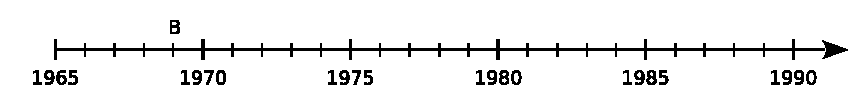
\includegraphics[width=\linewidth]{axe1965-1990}

Ce nombre est associé à un événement historique important. Lequel ?
Décalque cette demi-droite et place le point $N$ associé au nombre qui correspond à l'année de la chute du mur de Berlin.

Le nombre associé à un point sur une demi-droite graduée est l'\textbf{abscisse} de ce point.

\end{partie}

\begin{partie}[Des partages de plus en plus petits]
\begin{enumerate}
 \item Reproduis et complète la demi-droite graduée ci-dessous. \label{NbEntDec_Acti1Qa}
 
 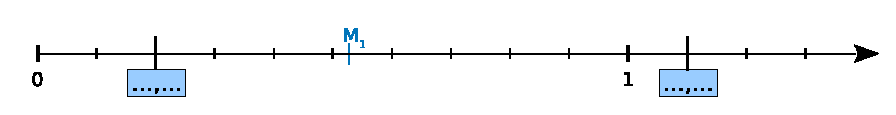
\includegraphics[width=\linewidth]{axe0-1}
 
 \item Détermine les abscisses des points $S$, $P$, $R$, $V$, $T$ et $U$ repérés en noir sur les demi-droites graduées ci-dessous.\label{NbEntDec_Acti1Qb}
 
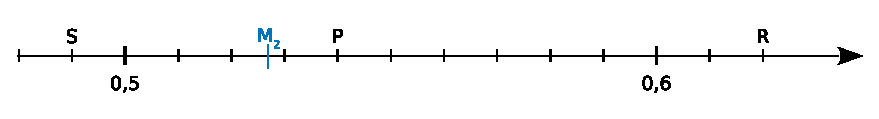
\includegraphics[width=\linewidth]{axe05-06}

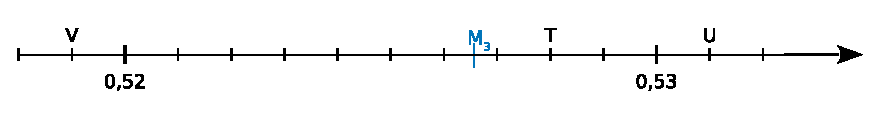
\includegraphics[width=\linewidth]{axe052-053}
 
 \item Sur une demi-droite, graduée judicieusement, place précisément les points $X$ et $Y$ d'abscisses respectives $0,526\,5$ et $0,527\,1$.
 \item Donne un \textbf{encadrement}, le plus précis possible, de l'abscisse des points $M_1$, $M_2$ et $M_3$ repérés en bleu sur les demi-droites graduées des questions \ref{NbEntDec_Acti1Qa} et \ref{NbEntDec_Acti1Qb}.
 \end{enumerate}
\end{partie}

\end{activite}


%%%%%%%%%%%%%%%%%%%%%%%%%%%%%%%%%%%%%%%%%%%%%%%%%%%%%%%%%%%%%%%%%%%%%%%%


\begin{activite}[L'écriture décimale]
\begin{enumerate}
 \item 349,785 est un nombre noté en écriture décimale. Dans ce nombre, quel est le chiffre représentant les unités ? Que désigne le chiffre 7 ? Et le chiffre 8 ?
 \item Le nombre 123,409 peut se lire « 123 virgule 409 ». Donne une autre lecture possible en utilisant les mots unités, dixièmes, centièmes et millièmes.
Que représente chacun des chiffres de ce nombre ? 4 est-il le chiffre des centaines ?
 \item Combien de centièmes y a-t-il dans un  dixième ? Dans une  unité ?
Combien de millièmes y a-t-il dans un centième ? Dans un dixième ? Dans une unité ?
 \item Combien de centièmes y a-t-il dans 7 unités 4 dixièmes ? Et dans 25 unités 8 dixièmes et 7 centièmes ?
 \end{enumerate}
\end{activite}


%%%%%%%%%%%%%%%%%%%%%%%%%%%%%%%%%%%%%%%%%%%%%%%%%%%%%%%%%%%%%%%%%%%%%%%%


\begin{activite}[Comparer, ranger et intercaler]

\begin{partie}[Comparer et ranger]
\begin{enumerate}
 \item Lequel des deux nombres 0,85 et 1,2 est le plus proche de 1 ? Quel est le nombre le plus proche de $12 : 11,9$ ou 12,08 ? Justifie avec soin tes réponses.
 \item Range les nombres de chaque liste dans l'ordre \textbf{croissant} (c'est-à-dire du plus petit au plus grand).
 	\begin{itemize}
	\item 1\,250 ; 1\,025 ; 125 ; 15\,200 ; 1\,520 ; 5\,120 ; 12\,500 ; 10\,520
	\item $10 + 0,5 + 0,06$ ; $7 + 0,5$ ; $10 + 0,06$ ; $7 + 0,05$ ; $10 + 0,6$ et $7 + 0,04 + 0,006$
	 \end{itemize}
 \item On a représenté ci-dessous une partie d'une demi-droite graduée.
 
 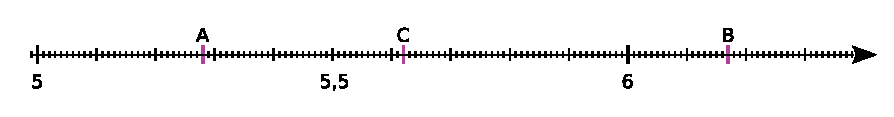
\includegraphics[width=\linewidth]{axe5A-6B}

Quelles sont les abscisses des points $A$, $B$ et $C$ ?

\vspace{0.75em}

Reproduis sur du papier millimétré cette portion de demi-droite et place les points $D$, $E$, $F$ et $G$ d'abscisses respectives 5,4 ; 6,22 ; 5,9 et 5,49.
Range alors les abscisses des points $A$, $B$, $C$, $D$, $E$, $F$ et $G$ dans l'ordre \textbf{décroissant}.
 \item À l'aide des questions précédentes et de tes connaissances, explique pourquoi les raisonnements d'élèves suivants ne sont pas justes et donne les raisons qui ont pu motiver leurs erreurs.
	\begin{itemize}
	\item \emph{« 24,5 < 6,08 car 245 < 608. »}
	\item \emph{« 19,85 < 12,96 car 0,85 < 0,96. »}
	\item \emph{« 6,012 > 6,35 car, à \textbf{partie entière} égale, le plus grand nombre est celui qui a le plus de chiffres après la virgule. »}
	\item \emph{« 5,24 > 5,8 car les parties entières sont égales et 24 > 8. »}
	\item \emph{« 14,3 < 14,30 car les parties entières sont égales et 3 < 30. »}
	\item \emph{« 103,6020 = 13,62 car les zéros ne servent à rien. »}
	\item \emph{« 16,295 < 16,38 car les parties entières sont égales et 16,295 a plus de chiffres après la virgule que 16,38. »}
	 \end{itemize}
 \end{enumerate}
\end{partie}

\begin{partie}[Intercaler]
\begin{enumerate}
 \item Quel est le nombre entier qui suit 128 ? Est-il possible de répondre à cette question si l'on remplace entier par décimal ?
Mêmes questions si on remplace 128 par 5,4.
 \item Est-il possible de trouver un nombre entier compris entre 1\,025 et 1\,026 ? Si oui, donne un exemple.
Même question en remplaçant « nombre entier » par « nombre décimal ».
 \item Est-il possible de trouver un nombre décimal compris entre 12,88 et 12,89 ? Et entre 8,975 et 8,976 ?
 \item À ton avis, est-il toujours possible de trouver plusieurs nombres décimaux compris entre deux nombres décimaux ?
 \end{enumerate}
\end{partie}

\end{activite}


%%%%%%%%%%%%%%%%%%%%%%%%%%%%%%%%%%%%%%%%%%%%%%%%%%%%%%%%%%%%%%%%%%%%%%%%

\begin{activite}[Multiplication et division par 10 ; 100 ; 1000 \ldots]

\begin{partie}[Multiplication par 10 ; 100 ; 1000 \ldots]
Le nombre 924,65 est égal à 9 centaines plus 2 dizaines plus 4 unités plus 6 dixièmes plus 5 centièmes.
\begin{enumerate}
 \item On veut multiplier par 10 le nombre suivant : 7 centaines plus 8 dizaines plus 3 unités plus 5 dixièmes plus 4 centièmes. Écris le résultat sous la même forme puis déduis-en une égalité en écriture décimale. \label{NbEntDec_Acti4Qa}
 \item Écris le nombre 15,034 comme dans la question \ref{NbEntDec_Acti4Qa}. Multiplie‑le par 1\,000 en t'inspirant de la question précédente.
 \item Donne une règle permettant de multiplier un nombre décimal par 10, 100 ou 1\,000. Que devient cette règle dans le cas d'un nombre entier ?
 \end{enumerate}
\end{partie}

\begin{partie}[Division par 10 ; 100 ; 1000 \ldots]
\begin{enumerate}
 \item En t'inspirant de la méthode précédente, divise par 10 le nombre 3 milliers plus 4 dizaines plus 6 unités plus 3 dixièmes plus 5 centièmes. Écris l'égalité en écriture décimale. \label{NbEntDec_Acti4Qa_2}
 \item Écris le nombre 73,305 comme dans la question \ref{NbEntDec_Acti4Qa_2} puis divise‑le par 1\,000.
 \item Donne une règle permettant de diviser un nombre décimal par 10, 100 ou 1\,000.
 \end{enumerate}
\end{partie}

\end{activite}


%%%%%%%%%%%%%%%%%%%%%%%%%%%%%%%%%%%%%%%%%%%%%%%%%%%%%%%%%%%%%%%%%%%%%%%%

\begin{activite}[Techniques opératoires]

\begin{partie}[Addition et soustraction de nombres décimaux]
\begin{enumerate}
 \item Pose et effectue l'opération $123,67 + 2,655$. Explique la méthode.
 \item Domitille et Virgile ont effectué cette opération et voilà ce qu'ils ont trouvé :\\[0.5em]
 
 \begin{minipage}[t]{.44\linewidth} 
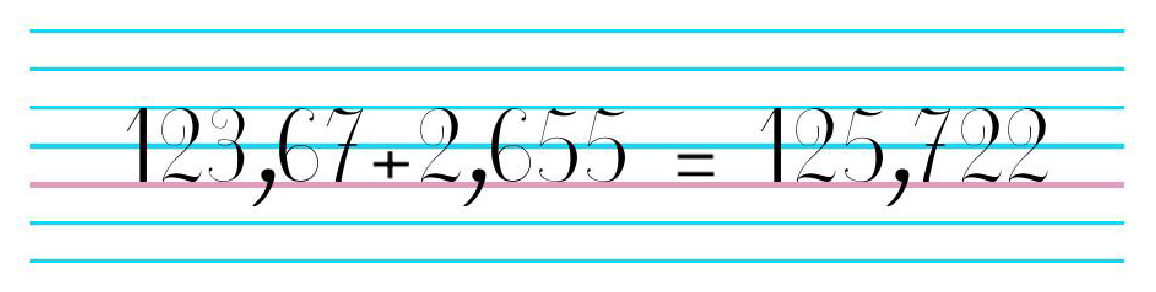
\includegraphics[width=5.5cm]{rep_domitille}
 \end{minipage}\hfill%
 \begin{minipage}[t]{.56\linewidth}
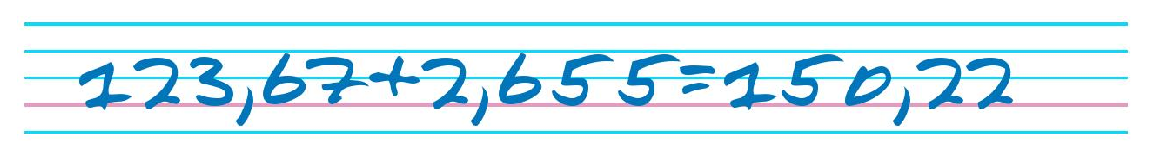
\includegraphics[width=7.5cm]{rep_virgile}
 \end{minipage}\\
  \begin{minipage}[t]{.44\linewidth} 
\begin{center} Réponse de Domitille \end{center}
 \end{minipage}\hfill%
 \begin{minipage}[t]{.56\linewidth}
\begin{center} Réponse de Virgile \end{center}
 \end{minipage}\\
 
 Que penses‑tu de leurs résultats ? Explique leurs éventuelles erreurs.
 \item Ambre était absente le jour où la maîtresse a expliqué comment on soustrait des nombres décimaux. Écris un texte le lui expliquant, donne un exemple.
 \end{enumerate}
\end{partie}

\begin{partie}[Multiplication d'un nombre décimal par un nombre entier]
\begin{enumerate}
 \item Pose et effectue l'opération $123,7 + 123,7 + 123,7 + 123,7$.
 \item Pose et effectue l'opération $123,7 \cdot 4$. Compare les deux opérations.
 \item Pose et effectue l'opération $52,8 \cdot 6$.
 \item Lucas a noté une série d'opérations pour calculer $52,8 \cdot 6$ : \\[-1em]
 
 $0,8 \cdot 6 = 4,8$ \hfill $2 \cdot 6 = 12$ \hfill $50 \cdot 6 = 300$ \hfill $300 + 12 + 4,8 = 316,8$ \\[-1em]
 
 Que penses‑tu de cette méthode ?
 \item Effectue l'opération $763,6 \cdot 3$ en utilisant la méthode de Lucas puis pose‑la pour vérifier ton résultat.
 \item Adapte cette méthode pour effectuer l'opération $1,34 \cdot 18$. Pose ensuite l'opération pour vérifier ton résultat.
 \end{enumerate}
\end{partie}

\end{activite}


%%%%%%%%%%%%%%%%%%%%%%%%%%%%%%%%%%%%%%%%%%%%%%%%%%%%%%%%%%%%%%%%%%%%%%%%



\begin{activite}[Vérifier un résultat]

\begin{enumerate}
 \item Sans poser aucune opération et sans utiliser de calculatrice, associe chaque calcul de gauche à un résultat de droite. \\[0.5em]
 
\begin{minipage}[t]{0.48\linewidth}
\begin{center}
\begin{ttableau}{0.7\linewidth}{1}
\hline \rowcolor{B3} \textbf{a.} $\quad 56 \cdot 123$ \\
\hline \rowcolor{G3} \textbf{b.} $\quad 12,35 + 1,68$ \\
\hline \rowcolor{B3} \textbf{c.} $\quad 1\,073 : 200$ \\
\hline \rowcolor{G3} \textbf{d.} $\quad 0,255 + 0,728$ \\
\hline \rowcolor{B3} \textbf{e.} $\quad 0,255 \cdot 0,728$ \\
\hline \rowcolor{G3} \textbf{f.} $\quad 13,23 : 5$ \\
\hline \rowcolor{B3} \textbf{g.} $\quad 520 \cdot 36$ \\
\hline \rowcolor{G3} \textbf{h.} $\quad 428 + 537$ \\
\hline \rowcolor{B3} \textbf{i.} $\quad 1,2 \cdot 2,4$ \\
\hline \rowcolor{G3} \textbf{j.} $\quad 18 \cdot 29$ \\
\hline
\end{ttableau}
\end{center}
\end{minipage} \hfill%
\begin{minipage}[t]{0.48\linewidth}
\begin{center}
\renewcommand*\tabularxcolumn[1]{>{\centering\arraybackslash}m{#1}}
\begin{ttableau}{0.6\linewidth}{1}
\hline \rowcolor{H3} 5,365 \\
\hline \rowcolor{J3} 2,88 \\
\hline \rowcolor{H3} 6\,888 \\
\hline \rowcolor{J3} 0,983 \\
\hline \rowcolor{H3} 2,646 \\
\hline \rowcolor{J3} 965 \\
\hline \rowcolor{H3} 522 \\
\hline \rowcolor{J3} 14,03 \\
\hline \rowcolor{H3} 18\,720 \\
\hline \rowcolor{J3} 0,185\,64 \\
\hline
\end{ttableau} 
\end{center}
 \end{minipage} \\
 
 \item Explique le plus précisément possible la manière dont tu as trouvé les résultats.\label{NbEntDec_Acti6Q2}
 \item Maverick a effectué des calculs ci-dessous. Détermine quels résultats sont forcément faux en utilisant les méthodes décrites à la question \ref{NbEntDec_Acti6Q2}.\\[1em]
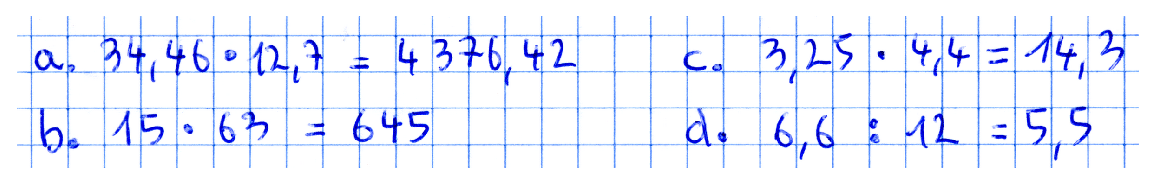
\includegraphics[width=\linewidth]{calcul_Maverick}

 \end{enumerate}
 
 \end{activite}


%%%%%%%%%%%%%%%%%%%%%%%%%%%%%%%%%%%%%%%%%%%%%%%%%%%%%%%%%%%%%%%%%%%%%%%%


